\definecolor{cof}{RGB}{219, 144, 71}
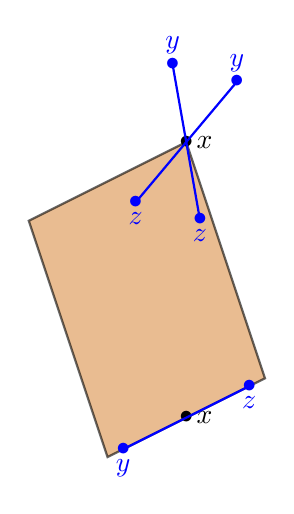
\begin{tikzpicture}[thick]
  \coordinate (A1) at (0, 0);
  \coordinate (A2) at (2, 1);
  \coordinate (A3) at (1, 4);
  \coordinate (A4) at (-1, 3);
  
  \draw[fill=cof, opacity=0.6] (A1) -- (A2) -- (A3) -- (A4) --cycle;
  \draw (A3) node {$\bullet$} node[right] {$x$} ;
  \draw[blue] (A3) -- ++(50:1) node {$\bullet$} node[above] {$y$};
  \draw[blue] (A3) -- ++(230:1) node {$\bullet$} node[below] {$z$};
  \draw[blue] (A3) -- ++(100:1) node {$\bullet$} node[above] {$y$};
  \draw[blue] (A3) -- ++(280:1) node {$\bullet$} node[below] {$z$};
  \draw (1, 0.5) node {$\bullet$}  node[right] {$x$} ;
  \draw[blue] (0.2, 0.1) node {$\bullet$}  node[below]
       {$y$} -- (1.8, 0.9) node {$\bullet$} node[below] {$z$};
\end{tikzpicture}
